\section{Final Unity structure}
Two scenes have been created in Unity: \textit{StartMenu} and \textit{Main}.
This section will give an overview of these two scenes, and show the game objects that have been used in this project.

\subsection{Start menu}
The start menu is the lobby and the game objects within the scene can be seen on \autoref{fig:startmenu-game-objects}.

\begin{figure}[H]
    \centering
    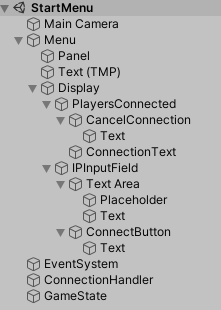
\includegraphics[width=0.4\linewidth]{figures/startmenu.PNG}
    \caption{The game objects in the start menu.}
    \label{fig:startmenu-game-objects}
\end{figure}
\noindent
The five main game objects are the \texttt{GameStateHandler}, \texttt{ConnectionHandler}, \texttt{EventSystem}, \texttt{Menu}, and the standard \texttt{Main Camera}.
\\
The \texttt{GameState} contains a simple script with information relating to the state of the game, such as anchor positions, player positions and other different variables used when the game starts.
It also contains another script called \texttt{DontDestroy}, which ensures that the game object does not get destroyed when changing scene, such that information received while on the menu can be accessed during play in the game.
\\
\texttt{ConnectionHandler} contains the scripts \texttt{DontDestroy} and \texttt{TCPClient}.
The \texttt{TCPClient} receives the information from the host and adds the information received to the \texttt{GameState}.
\\
\texttt{Menu} has multiple game objects as children, which are used to specify how the UI should look.
Menu also has a script which disables virtual reality in this scene.
The menu is not intended to be in virtual reality, as the IP address has to be inputted.
The \texttt{ConnectButton} and \texttt{CancelConnection} buttons use an \texttt{OnClick} feature in Unity, where it calls a function to either connect or cancel the connection, which also changes the UI to reflect this.
\\
The \texttt{EventSystem} supports sending events to objects based on input as clicks on buttons or typing in the text field.

\subsection{Main scene}
The main scene is the game scene with the playing field.
The primary objects in the main scene are \texttt{CLIENT}, \texttt{PlayingFieldContainer}, \texttt{Camera Rig} and \texttt{GvrEventSystem}.
These can be seen on \autoref{fig:main-game-objects}.\begin{figure}[H]
    \centering
    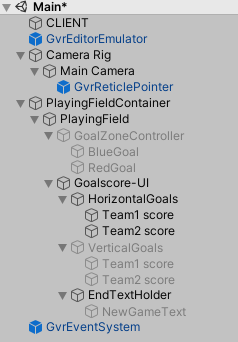
\includegraphics[width=0.4\linewidth]{figures/unity-main-gameobjects.PNG}
    \caption{The game objects in the main game scene. The grey game objects are not active and the blue are prefabs.}
    \label{fig:main-game-objects}
\end{figure}
\noindent
The \texttt{CLIENT} contains the script \texttt{UDPClient}, which instantiates the UDP client and receives player and ball positions.
This script is previously described in \autoref{sec:receiving-the-information}.
\\
The \texttt{PlayingFieldContainer} only has \texttt{PlayingField} as a child and has the script \texttt{CameraFollow} attached.
This script ensures that the playing field is always in the center of the camera.
The \texttt{PlayingField} has two children, where one of them is the texttt{GoalZoneController}, which is used to generate the playing field and make sure that the entire field is visible by the camera.
The other is the \texttt{Goalscore-UI}, which is used to display the current score of the game.
The playing field has two scripts attached, \texttt{FieldGenerator} and \texttt{PlayingFieldOffset}.
\texttt{FieldGenerator} creates the playing field from the coordinates in the \texttt{GameStateHandler}, which was instantiated in the lobby.
\texttt{PlayingFieldOffset} is used to change the center coordinate of the field, so that it has the same $x$ and $y$ position as the camera.
This is a requirement because of the way meshes are rendered in Unity.
Rather than being aligned by their center, they are aligned by default by their bottom left corner.
As such, to keep the playing field in view, it must have this offset.
